\documentclass{standalone}
\usepackage{pgfplots}
\pgfplotsset{compat=1.18}
\usepgfplotslibrary{colorbrewer}
\pgfplotsset{cycle list/Set1-6}

\begin{document}

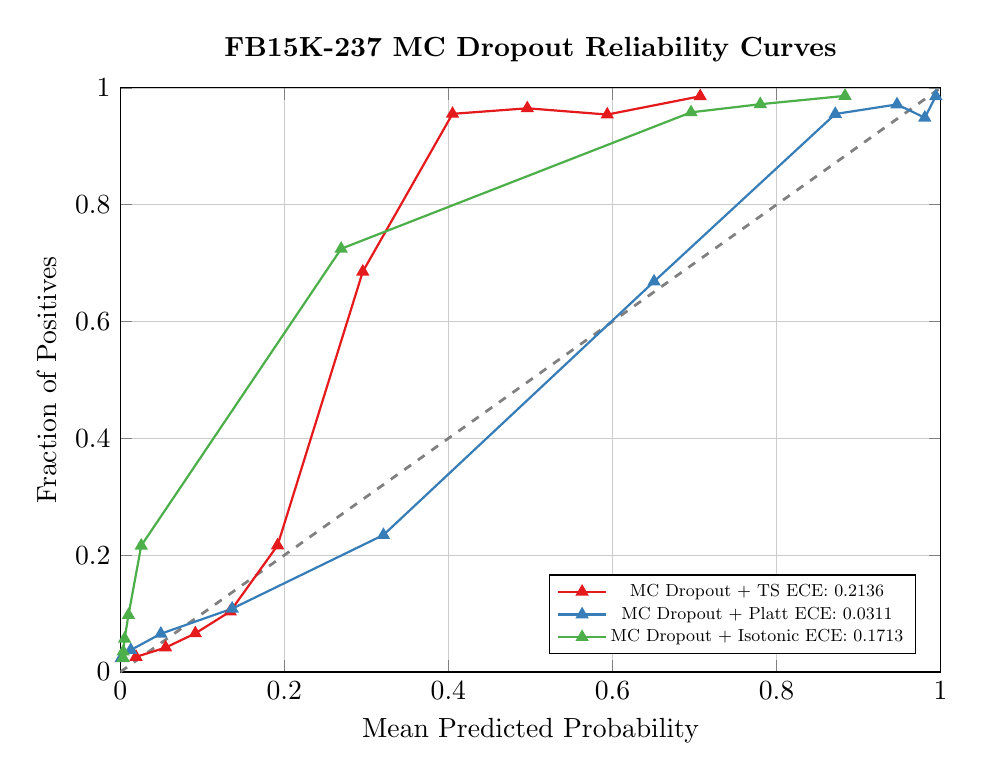
\begin{tikzpicture}
\begin{axis}[
    title={\textbf{FB15K-237 MC Dropout Reliability Curves}},
    xlabel={Mean Predicted Probability},
    ylabel={Fraction of Positives},
    xmin=0, xmax=1,
    ymin=0, ymax=1,
    xtick={0, 0.2, 0.4, 0.6, 0.8, 1.0},
    ytick={0, 0.2, 0.4, 0.6, 0.8, 1.0},
    legend pos= south east,
    legend style={nodes={scale=0.7, transform shape}, font=\small},
    grid=both,
    grid style={line width=.1pt, draw=gray!20},
    major grid style={line width=.2pt, draw=gray!40},
    width=12cm,
    height=9cm,
    cycle list name=Set1-6
]

% Perfectly Calibrated Line
\addplot [color=gray, dashed, line width=1pt, forget plot]
    coordinates {(0,0)(1,1)};

\addplot+[mark=triangle*, thick] coordinates {
    (0.01916377, 0.02589155) (0.05528829, 0.04177865) (0.09153946, 0.06621060) 
    (0.13403509, 0.10359150) (0.19175528, 0.21671146) (0.29562051, 0.68531639) 
    (0.40502768, 0.95553384) (0.49620390, 0.96506230) (0.59367061, 0.95431224) 
    (0.70696172, 0.98558867)
};
\addlegendentry{MC Dropout + TS ECE: 0.2136}


\addplot+[mark=triangle*, thick] coordinates {
    (0.00121503, 0.02369321) (0.01280660, 0.03762521) (0.04945199, 0.06547764) 
    (0.13640896, 0.10847789) (0.32080918, 0.23454679) (0.65068354, 0.66845834) 
    (0.87161947, 0.95528952) (0.94684374, 0.97165893) (0.98071578, 0.94893721) 
    (0.99419234, 0.98583293)
};
\addlegendentry{MC Dropout + Platt ECE: 0.0311}


\addplot+[mark=triangle*, thick] coordinates {
    (0.00354425, 0.02418173) (0.00361810, 0.03493770) (0.00529614, 0.05692646) 
    (0.01000929, 0.09750353) (0.02558703, 0.21631206) (0.26926836, 0.72456747) 
    (0.69578898, 0.95813772) (0.78021818, 0.97203728) (0.88347345, 0.98628634)
};
\addlegendentry{MC Dropout + Isotonic ECE: 0.1713}

\end{axis}
\end{tikzpicture}

\end{document}